%----------------------------------------
\chapter{\analysis}\label{chap:analysis}
%----------------------------------------
A dolgozat során elkészített rendszer terv csak akadémiai célokat szolgál, ezért nem követi teljes mértékben a valóságot.
Teljes mértékben kielégítő biztonsági vizsgálatot ezért nem lehet végezni a rendszeren.
A következő részekben inkább szeretném bemutatni egyes elemzési módszerek lényegét, alkalmazhatóságát mintsem egy valós projekt szerinti precíz megvalósítsát.

Mivel a biztonságosság kiemelten fontos témakör az iparágban, ezért az elemzésben a valósághoz hasonló értékek szerepelnek, de ezen értékek kitaláltak és reprezentatív jellegűek.
Az analízis során feltárt kockázatok besorolását az EN 50126\cite{EN50126-1} első részében leírt kockázat mátrix kalibrációs táblázatai szerint határoztam meg.

A frekvenciák besorolásához a \ref{tab:freqency}. táblázatot készítettem el.
Ennek segítségével besorolhatók egyes kvantitatív értékek az elfogadási mátrixban.

Továbbá a \ref{tab:serverity} és a \ref{tab:risk} segédtáblázatok alapján már meghatározható az a táblázat, amely a balesetek súlyossága és a hiba előfordulásának gyakorisága alapján meghatározza a kockázat elfogadásának lehetőséget.
Ezt a táblázatot reprezentálja a \ref{tab:risk_mat} táblázat.

Az elemzések további szakaszaiban ezen táblázatok felhasználása szerint lesznek meghatározva az előforduló hibák.
Továbbá feltételezhetjük, hogy a rendszer várható élettartama 30 év és átlagosan évente 5 000 órányi igénybevételnek lesz kitéve.

\begin{table}
    \footnotesize
    \centering
    \begin{tabular}{ |c|p{10em}|p{8em}|p{10em}| }
        \hline
        Frekvencia szint & Leírás & Frekvencia példa egy 24 órában működő eszköznél & Frekvencia \\
        \hline
        Gyakori & Az esemény gyakran bekövetkezik & Több mint egyszer 6 hónapos időszak alatt & $f \leq 1\times10^{-3}$ \\
        \hline
        Valószínű & Az esemény várhatóan többször bekövetkezik & Hozzávetólegesen egyszer 6 hét és egy év között & $ 1\times10^{-3} < f \leq 1\times10^{-4} $ \\
        \hline
        Alkalmi&Az esemény több alkalommal bekövetkezhet & Hozzávetőlegesen egyszer egy év és 10 év között & $1\times10^{-4} < f \leq 1\times10^{-5}$ \\
        \hline
        Ritka&Valószínű, hogy bekövetkezik valamikor a rendszer élettartama során & Hozzávetőlegesen egyszer 10 év és 1 000 év között & $1\times10^{-5} < f \leq 1\times10^{-7}$ \\
        \hline
        Valószínűtlen&Velószínűtlen a bekövetkezés, de megtörténhet & Hozzávetőlegesen egyszer 1 000 év és 100 000 év között & $1\times10^{-7} < f \leq 1\times10^{-9}$ \\
        \hline
        Erősen valószínűtlen&Az esemény vélhetően egyszer sem fog bekövetkezni & Hozzávetőlegesen egyszer 100 000 éveben vagy kevesebbszer & $1\times10^{-9} < f$ \\
        \hline
    \end{tabular}
    \caption{A veszély besorolási mátrix frekvencia tartomány kalibrációja. Saját adatok, a \cite{EN50126-1} alapján.}
    \label{tab:freqency}
\end{table}

\begin{table}
    \footnotesize
    \centering
    \begin{tabular}{ |c|p{10em}|p{10em}| }
        \hline
        Súlyossági kategória & Következmények az emberekre / környezetre                                                                                                     & Következmények a szolgáltatásokra \\ \hline
        Katasztrofális       & Emberek tömegét befolyásolja és többek halálához vezethez és/vagy  súlyos környezeti károsodás      & -                                 \\ \hline
        Kritikus             & Emberek kis számát befolyásolja és legalább egy halálesetet okoz és/vagy  nagy környezeti károsodás & Egy fontos rendszer elvesztése    \\ \hline
        Marginális           & Nincs lehetőség halálesetre, cask súlyos vagy könnyű sérülések és/vagy kis környezeti károsodás     & Súlyos rendszer sérülés           \\ \hline
        Jelentéktelen        & Lehetséges könnyű sérülés                                                                                                                     & Jelentéktelen rendszer sérülés    \\ \hline
    \end{tabular}
    \caption{Súlyossági kategóriák, az EN 50126-1 alapján.}
    \label{tab:serverity}
\end{table}

\begin{table}
    \footnotesize
    \centering
    \begin{tabular}{ |c|p{20em}| }
        \hline
        Kockázat elfogadási kategória & Végrehajtandó intézkedések\\ \hline
        Tolerálhatatlan & A kockázatot meg kell szüntetni \\ \hline
        Nem kívánatos & A kockázatot csak abban az esetben lehet elfogadni, ha annak csökkentése nem lehetséges \\ \hline
        Tolerálható & A kockázat tolerálható és elfogadható megfelelő ellenőrzéssel (például: karbantartási útmutatók vagy szabályok) \\ \hline
        Elhanyagolható & A kockázat minden további nélkül elfogadható \\ \hline
    \end{tabular}
    \caption{Kockázat elfogadási kategóriák, az EN 50126-1 alapján.}
    \label{tab:risk}
\end{table}

\begin{table}
    \centering
    \begin{tabular}{|l|l|l|l|l|} 
        \hline
        Előfordulási frekvencia & \multicolumn{4}{l|}{Kockázat elfogadási kategória}                    \\ 
        \hline
        Gyakori                 & Nem kívánatos  & Tolerálhatatlan & Tolerálhatatlan & Tolerálhatatlan  \\ 
        \hline
        Valószínű               & Tolerálható    & Nem kívánatos   & Tolerálhatatlan & Tolerálhatatlan  \\ 
        \hline
        Alkalmi                 & Tolerálható    & Nem kívánatos   & Nem kívánatos   & Tolerálhatatlan  \\ 
        \hline
        Ritka                   & Elhanyagolható & Tolerálható     & Nem kívánatos   & Nem kívánatos    \\ 
        \hline
        Valószínűtlenű          & Elhanyagolható & Elhanyagolható  & Tolerálható     & Nem kívánatos    \\ 
        \hline
        Erősen valószínűtlen    & Elhanyagolható & Elhanyagolható  & Elhanyagolható  & Tolerálható      \\ 
        \hline
        \multicolumn{1}{l|}{}   & Jelentéktelen  & Merginális      & Kritikus        & Katasztrofális   \\ 
        \cline{2-5}
        \multicolumn{1}{l|}{}   & \multicolumn{4}{l|}{A baleset súlyossága}                             \\
        \cline{2-5}
        \end{tabular}
    \caption{Kockázat elfogadási mátrix.}
    \label{tab:risk_mat}
\end{table}

\section{HAZOP analízis}
A vizsgálatot HAZOP tanulmány készítésével kezdtem.
Ez alkalmas a rendszer platform modellje alapján előre meghatározott módszertan szerint szisztematikusan eltárni az adott alrendszerek tervezettől való eltérő viselkedéseinek feltárására.

A vizsgálat segéd szavak segítségével vezeti rá az elemző (csapat) gondolkodását a lehetséges eltérésekre.
A módszertan által nyújtott lehetséges szavak csak egy részét felhasználva, a következő iránymutató szavak lettek felhasználva a dolgozatban: (1) NEM (NO), (2) KEVESEBB (LESS), (3) TÖBB (MORE).

Ezután két alrendszert vizsgáltam a módszertan szerint, ezek pedig a hidraulikus fékolló (Hydraulic Caliper) és a vezérlő elektronika (Control Electronics).

A HAZOP tanulmány eredményessége nagyban függ az azt végrehajtó csapat kreativitásán, ezért nem feltételezhető az adott egység minden egyes hibaforrásának észlelése/feltárása.

Az általam elvégzett vizsgálat során a \ref{tab:hazop_vizsg}. táblázatban látható potenciális eltérésekre jutottam.


\begin{table}
    \centering
    \begin{tabular}{ |p{18mm}|p{15mm}|p{20mm}|p{20mm}|p{25mm}|p{25mm}| }
        \hline
        Item & Guide word & Deviation & Cause & Consequence & Existing controls \\
        \hline
        Hydraulic Caliper & NO & No brake force & Caliper failure & Longer braking distance / possible crash with traffic & Recommended service interval / routine checks \\
        & LESS & Reduced brake force & Worn out brakepads & Longer braking distance / possible crash with traffic & Recommended service interval / routine checks \\
        & LESS & Reduced brake force & Control loop failure & Longer braking distance / possible injury to multiple people & - \\
        & MORE & More brake force & Failure of pressure generation & Possibility of train stuck on track / minor injuries & - \\
        \hline
        Control Electronics & NO & No input voltage & Train battery line failure & Train stuck on track & - \\
        & MORE & Higher input voltage than specified & Train battery line failure & Control electronics power supply failure & Over voltage protection \\
        & MORE & Higher brake demand than requested & Control output stuck at low & Possibility of train stuck on track / minor injuries & Under voltage protection \\
        & LESS & Lower input voltage than specified & Train battery line failure & Possibility of train stuck on track / minor injuries & - \\
        & LESS & Lower brake demand than requested & Control output stuck at high & Longer braking distance / possible injury to multiple people & Error signaling \\
        & LESS & Lower brake demand than requested & Wheelslide protection lowers the brake demand for a long time & Longer braking distance / possible injury to multiple people & WSP watchdog \\
        \hline
    \end{tabular}
    \caption{HAZOP vizsgálat a hidraulikus fékolló és vezérlő elektronika komponensekre.}
    \label{tab:hazop_vizsg}
\end{table}

\section{LOPA analízis}
A LOPA vizsgálat során a következő forgatókönyvet fogom elemezni: A kerékcsúszás prevenciós modul túl sokáig (> 3 sec) tartja fékezetlen állapotban a rendszert miközben fékezési parancs van kiadva.

HAZOP tanulmány során derült fény erre a potenciális hibára. 
A tanulmány alapján kijelenthető, hogy a eset kiváltó hiba potenciálisan a kerékcsúszás prevenciós alrendszer beragadása egy olyan állapotba, ahol jelentősen csökkentett fékerő kerül kivezérlésre a végős beavatkozóhoz.

Ez különböző módokon lehetséges, amiknek további elemzése nem célja a vizsgálatnak, de lehet processzor, memória esetleg a vezérlést végrehajtó hardver hibája.
Továbbá tudjuk, hogy ez a hiba $4\times10^{-4} {1/h}$ frekvenciával fordul elő.

A lehetséges következmények között feltárva lett, olyan kimenetel is, hogy a hiba akár halálesethez is vezethet.
Ezért a \ref{tab:serverity} táblázat alapján a hiba \emph{Kritikus} besorolást kap.
A megadott hibarátát figyelembe véve a \ref{tab:freqency} táblázat szerint az előfordulás besorolása \emph{Alkalmi} kategóriájú.

A fentiek alapján a következő megállapítás fogalmazhatódhat meg az hibamód elfogadhatóságáról: A kapott besorolások alapján bármilyen enyhítő körülmény nélkül a kockázat elfogadási mátrix (lásd: \ref{tab:risk_mat}. táblázat) alapján \emph{Nem kívánatos} besorolást kap.
Ez csak akkor elfogadható, ha azt lehetséges tovább csökkenteni.

\subsection{Független Védelmi Rétegek vizsgálata}
Ahhoz, hogy eszközt, rendszert vagy funkciót független védelmi rétegnek (továbbiakban IPL\footnote{Independent Protection Layer}) lehessen tekinteni a következőnek kell teljesülni\cite{LOPABOOK}:
\begin{itemize}
    \item \emph{hatékonyan} megakadályozza következményt ha úgy működik, ahogy tervezték
    \item \emph{független} a kezdő/kiváltó eseménytől és a többi IPL összes komponensétől, ami szerepel a forgatókönyvben
    \item \emph{auditálható}, az elvárt viselkedés valamilyen módon validálható/bizonyítható
\end{itemize}

Az IPL-eknek két altípusát különböztetjük meg: (1) Passzív IPL, (2) Aktív IPL.

A passzív IPL-eknek nem szükséges, hogy beavatkozzanak a folyamatba ők eredendően csökkentik a kockázatot.
Az irodalomban számtalan példa található a kémiai iparágban használható passzív védelmi mechanizmusokról, de a jelen problémához nem alkalmazható ilyen elven működő eszköz.

Az aktív IPL-ek valamilyen érzékelő segítségével képes egyik állapotból a másikba kerülni ezáltal megváltoztatva a folyamatot.
Ezek egy lehetséges felépítését a \ref{fig:activeIPL}. ábra szemlélteti.
\begin{figure}
    \footnotesize
    \centering
    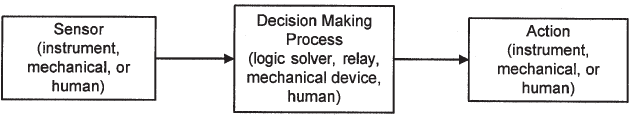
\includegraphics[width=100mm, keepaspectratio]{figures/lopa_active_IPL.png}
    \caption{Egy aktív IPL felépítése. Forrás: \cite{LOPABOOK}}
    \label{fig:activeIPL}
\end{figure}

A rendszer jelenlegi tervében sajnos nem szerepel ilyen elem. 
De szerencsére az iparágban található erre a problémakörbe megfelelő modul, amit fel lehet használni a probléma kiküszöbölésére.
Ez pedig a megfigyelő (watchdog) funkcionalitás, mely monitorozza a WSP\footnote{WheelSlide Protection} működését.

Az IPL-ek hatékonyságát az eléréskori hiba valószínűsége (PFD\footnote{Probability of Failure on Demand}) határozza meg.

\subsection{Frekvencia számítás}
Az esemény következményének frekvenciáját az alábbi egyenlettel lehet megadni:
\begin{equation}
    f^C = f^I\times\prod^{J}_{j=1}{{PFD}_j}
\end{equation}
\label{eq:lopa}
Ahol,

$f^C$ a kimenetel frekvenciája

$f^I$ a kezdeményező esemény frekvenciája és

$PDF_j$ a j-edik IPL hibájának valószínűsége, ami védelmet nyújt a kimenetellel szemben.

Néhányaknak szemetszúhatott már, hogy az IPL-ek esetében On-Demand hiba valószínűségről beszél a szakirodalom, míg a vasútiparban általában folytonos módban vannak megadva a tűrésértékek.
Ezért fontos kiemelni, hogy konverzió nélkül nem alkalmazható a fenti egyenlet.

A két szabványrendszer kapcsolatát a \ref{tab:sil_thr_pfd} táblázat írja le.
Mivel a rendszer tisztán elektronikus ezért a fejezet elején leírtak szerint a rendszer megbízhatósága $r(t) = e^{-\lambda t}$ közelíthető.
Továbbá szitén fentebb említettek szerint a rendszer élettartama 30 év, évi 5000 órás használattal.

Ezért annak a valószínűséget, hogy a rendszer meghibásodik az élettartama során (150 000 óra): $1-e^{-\lambda*150000}$
Ezt behelyettesítve a THR-rel megkapható az átlagos PFD értéke.

\begin{table}
    \footnotesize
    \centering
    \begin{tabular}{ |c|c|c| }
        \hline
        SIL besorolás & THR\footnote{Tolerable Hazard Rate} & PFD \\
        \hline
        SIL4 & $1e^{-8} < f \leq 1e^{-9}$ & $1e^{-3} < f \leq 1e^{-4}$ \\
        \hline
        SIL3 & $1e^{-7} < f \leq 1e^{-8}$ & $1e^{-2} < f \leq 1e^{-3}$ \\
        \hline
        SIL2 & $1e^{-6} < f \leq 1e^{-7}$ & $1e^{-1} < f \leq 1e^{-2}$ \\
        \hline
        SIL1 & $1e^{-5} < f \leq 1e^{-6}$ & $9e^{-1} < f \leq 1e^{-1}$ \\
        \hline
    \end{tabular}
    \caption{A SIL besorolások kapcsolata a THRrel és a PFDvel.}
    \label{tab:sil_thr_pfd}
\end{table}

A forgatókönyhöz tartozó tűrhető kockázat a fenti elemzésekből adodóan ${THR} > 1e^{-7}$.
A csökkentés nélküli frekvencia $1e^{-4}$, tehát a folyamat során legalább három nagyságrenddel kell csökkenteni a lehetséges előfordulást.

Ez úgy érhető el, ha a watchdog funkcióból SIF\footnote{Safety Instrumented Function}, azaz biztonság-kritikus funkció keletkezik SIL4-es besorolással, hiszen ekkor a fenti egyenlet szerint
\begin{align}
    \mathbf{f}^C&= \mathbf{f}^I\times \prod^{J}_{j=1}{\mathbf{PDF}_{j}} \\
     &= 1e^{-4}\prod 1e^{-3} \\
     &= 1e^{-7}
\end{align}
A csökkentett hibaelőfordulás már csak $f > 1e^{-7}$, ami tolerálható.

Ezért a vizsgálat utáni javaslat, hogy a folyamatot fel kell instrumentálni egy hibadetektáló alrendszerrel.
Továbbá, mivel egy SIL4-es funkció kifejlesztése nagyon költséges a vállaltra nézve és feltételezve, hogy a SIL2-es funkció ténylegesen képes két nagyságrendű csökkentésre lehetséges még egy modifikációs javaslat.
Néhány helyzetben költséghatékonyabb kifejleszteni két SIL2-es funkciót/terméket mint egy SIL4-est.
Ezek alapján a másik javaslat, hogy WSP funkcióból is képeznek egy SIF-et, amely így képes csökkenteni saját hibáit ezáltal az alap frekvenciát is.
Ha mind a WPS, mind a WPS watchdog részegységek SIL2-es besorolással rendelkeznek az eredő csökkentés $1e^{-4}$, amivel teljesíthető a tűrhető hibaráta követelménye.

\section{FTA}
A hibafa analízis az egyik legalaposabb és legáltalánosabb vizsgálati módszer.
Ha van olyan hibakövetkezmény, amit már az előzőleg végrehajtott módszerek felfedeztek, de bonyulultsága nem tette lehetővé, hogy részletesebben elemezzék akkor azt általában az FTA vizsgálja ki.

A dolgozatban ez a komplex alegység, melynek vizsgálatát erre a fejezetrészre hagytam, a vezérlő elektronika.
Ez az egység csak részben lett megemlítve az előző analízisek során és eddig a pontig csak annyit tudunk róla, hogy a WSP funkció, ami a mikroprocesszoron fut SIL2-es besorolást kapott.

\subsection{Kvalitatív analízis}
Ebben a részben azt a hibát kutatjuk - egyenlőre kvalitatív jellegel -, hogy mekkora valószínűséggel lesz detektálatlan hibamódban a vezérlő elektronika.

A részegység rendelkezik redundáns CAN kommunikációs interfésszel, amelyen képes adatokat fogadni és hibát is jelezni.
Az egész alaplap rendelkezik egy táppal, ami a vonat rendszerfeszültségéből képes a többi részegység által szükséges 5V feszültséget konvertálni.

Az alrendszer rendelkezik egy dedikált kommunikációs lehetőséggel, melyen a súlyos hibákat tudja jelezni a vonat szint (Train Level) felé. 
Elsődlegesen ez a hibajelző rendszer.

Továbbá, a vezérlési funkcióknak helyet adó mikroprocesszor található még az egységben.
Ez rendelkezik egy saját dedikált táppal, ami a $\mu C$-nek transzformálja a megfelelő feszültségszintet és a programkód számára elérhető memória modullal.

Ez alapján konstruálható olyan hibafa, ami a fent leírtak alapján helyezi el a hibamódokat.
Az elkészített hibafa a \ref{fig:qualit}. ábrán látható. Ezen látható, hogy nincsen teljesen normál formára hozva, hiszen a felső VAGY kapu alatt található még egy VAGY kapcsolat.
Ha teljesen normálalakúra alakítjuk az \emph{uC-FAILURE} kapu alatt lévő elemek egyenesen a Top-event alá kerülnek.
Így rendszerben hat darab minimális vágás található.

\begin{figure}
    \footnotesize
    \centering
    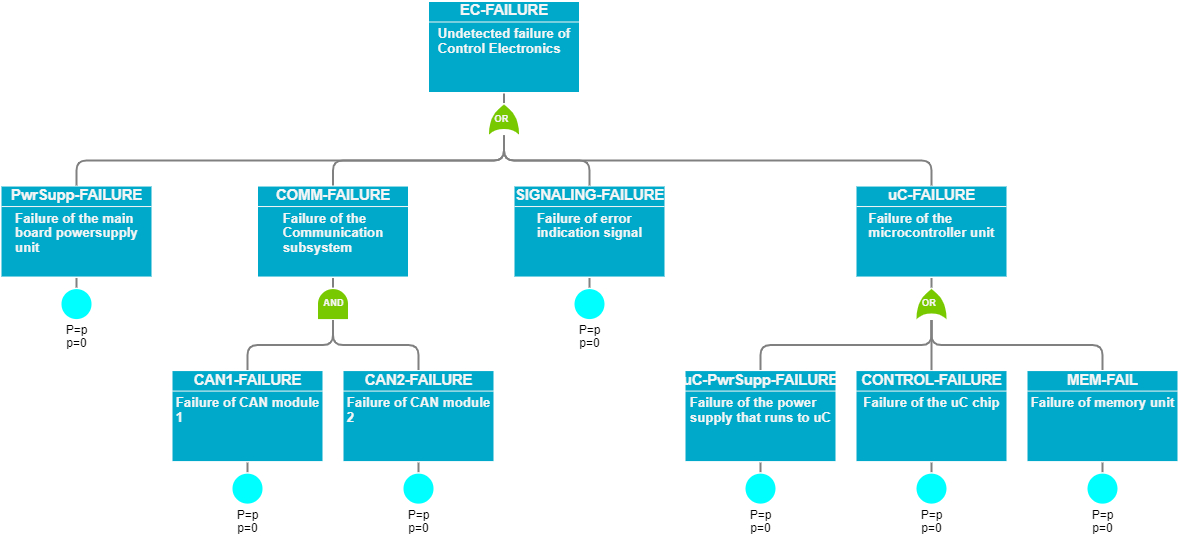
\includegraphics[width=150mm, keepaspectratio]{figures/QualitativeFTA.png}
    \caption{A vezérlőelektronika qualitatív hibafája.}
    \label{fig:qualit}
\end{figure}

\subsection{FIT allokáció}
A hibafa diagramm rendkívül alkalmas az alegységek logikai sorrendben reprezentálára.
Ezt kihasználva elvégezhetjük az EN 50129\cite{EN50129} által csak TFFR\footnote{Tolerable Functional Failure Rate} elosztását is.

Tegyük fel, hogy már meglévő vizsgálatok alapján és/vagy felsőbb utasítás hatására az a vezérlő elektronika SIL2-es besorolást kapott.
Ez azt jelentené, hogy maximum hibaráta amit az egység megengedhez, az $1e^{-6} \frac{1}{h}$.
Azt a felvetést követve, hogy a FIT\footnote{failure in time} az a $10^{9}$ órán belül történt hibák számát jelöli, a részegység 100 és 1000 FIT közötti értékből gazdálkodhat.

A SIL mellé megkaptuk, hogy a részegységnek 800 FIT-ből kell kigazdálkodni a teljes működését.

Ezt a 800 FIT-et kell elosztani az eggyel alacsonyabb szint felé osztani.
Most a már fentebbi fejezeketben említett egyenlő elosztási módszert alkalmazom, így minden alegységre 150 FIT jut, azaz a TFFR 150 FIT.

Mivel a kommunikációs modul két független részből áll, ezért a következő elvetés alkalmazható a további FIT allokációhoz: 
\begin{align}
    \mathbf{FFR}\approx 2{FR}^{2}\times {SDT}
\end{align}
ahol az SDT a safe down time-ot jelöli.

A képletet használva, 10 órás (nap végi ellenőrzés a detektáció) SDT-vel számolva elegendő lenne 8000 FIT-nek lennie minden egyes CAN csatornának.
De mivel ez kritikus funkciót valósít meg, ezért 800 FIT-et allokálok számukra (ami SIL2-es funkcionalitást jelent).

\subsection{Kvantitatív analízis}
A számolások során fiktív értékeket feltételezve a \ref{tab:fmeca} táblázatban szereplő értékekkel végzem.
Egy projekt során ezek az értékek egy FMECA analíziből származnának.

\begin{table}
    \footnotesize
    \centering
    \begin{tabular}{ |c|c|c| }
        \hline
        Item & FR(1/h) & P\_failure (150000h)\\
        \hline
        24V-5V supply & $1.5e^{-7}$&$2.22e^{-2}$ \\
        \hline
        CAN controller & $8e^{-7}$&$1.13e^{-1}$ \\
        \hline
        Signal control & $1.5e^{-7}$&$2.22e^{-2}$ \\
        \hline
        5V-1V2 supply & $1.5e^{-7}$&$2.22e^{-2}$ \\
        \hline
        $\mu$C & $1.5e^{-7}$&$2.22e^{-2}$ \\
        \hline
        Memory unit & $1.5e^{-7}$&$2.22e^{-2}$ \\ 
        \hline
    \end{tabular}
    \caption{Feladatban használt hibaráták és hiba valószínűsége}
    \label{tab:fmeca}
\end{table}

A valószínűségeket az alábbi egyenlet alapján lehet megkapni, a rendszer a fentebb meghatározott élettartama alapján: 
\begin{align}
    P&=1-e^{-\lambda t} \\
    &=1-e^{-150000\lambda}
\end{align}

\begin{figure}
    \footnotesize
    \centering
    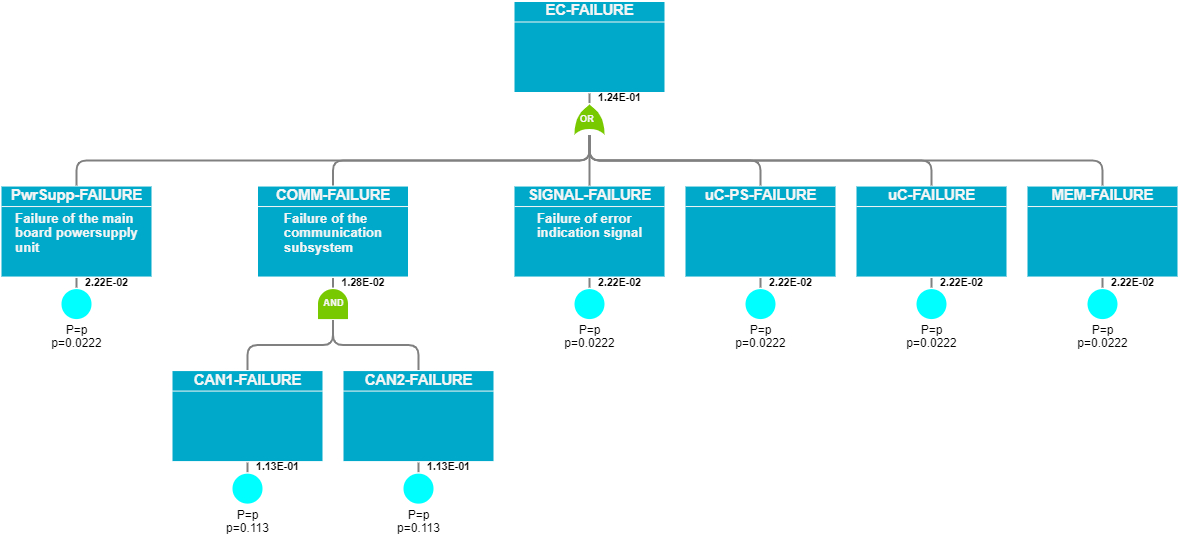
\includegraphics[width=150mm, keepaspectratio]{figures/QuantiFTA.png}
    \caption{Kvantitatív FTA az adott értékek alapján}
    \label{fig:quant}
\end{figure}

Amint az az \ref{fig:quant}. ábrán látható a kvantitatív analízis elvégzése után látható az alrendszer teljes élelttartamra számított detektálatlan hibájának a valószínűsége.
Ez sajnos nem egy szép alacsony szám, de vegyük figyelembe, hogy ez százötven-ezer órára vetített érték és még így is a rendszenszer számára allokált SIL kategóriába tartozik, sőt még a rendszer számára osztott TFFR-en is belül helyezkedik.
